% !TEX encoding = UTF-8
% !TEX program = pdflatex
% !TEX spellcheck = en_GB

\documentclass[english,a4paper]{europasscv}

\ecvname{Todor Dimitrov Balabanov}
\ecvaddress{dist. "Mladost" 1, bl. 18, et. 5, fl. 6, app. 16, \\ 1750 Sofia, Bulgaria}
\ecvtelephone[+359 89 8237103]{+359 2 8764645}
\ecvemail{todor.balabanov@gmail.com}
\ecvhomepage{linkedin.com/in/todor-balabanov}
%\ecvim{AOL Messenger}{todor.balabanov}
\ecvim{Google Talk}{todor.balabanov}

\ecvdateofbirth{12 February 1980}
\ecvnationality{Bulgarian}
\ecvgender{Male}

\ecvpicture[width=3.8cm]{picture.png}

\begin{document}
  \begin{europasscv}

  \ecvpersonalinfo

  \ecvbigitem{Job applied for}{Research team member}

  \ecvsection{Work experience}
  
  \ecvtitle{August 2002 -- Present}{Independent consultant}
  \ecvitem{}{British Council\newline 123, Bd Ney, 75023 Paris (France)}
  \ecvitem{}{Evaluation of European Commission youth training support measures for youth national agencies and young people}
   
  \ecvtitle{March 2002 -- July 2002}{Internship}
  \ecvitem{}{European Commission, Youth Unit, DG Education and Culture \newline 200, Rue de la Loi, 1049 Brussels (Belgium)}
  \ecvitem{}{
  \begin{ecvitemize}
      \item evaluating youth training programmes for SALTO UK and the partnership between the Council of Europe and European Commission
      \item organizing and running a 2 day workshop on non-formal education for Action 5 large scale projects focusing on quality, assessment and recognition
      \item contributing to the steering sroup on training and developing action plans on training for the next 3 years. Working on the Users Guide for training and the support measures
  \end{ecvitemize}
  }
  \ecvitem{}{\ecvhighlight{Business or sector}\quad European institution}
  
  \ecvtitle{Oct 2001 -- Feb 2002}{Researcher / Independent Consultant}
  \ecvitem{}{Council of Europe, Budapest (Hungary)}
  \ecvitem{}{Working in a research team carrying out in-depth qualitative evaluation of the 2 year Advanced Training of Trainers in Europe using participant observations, in-depth interviews and focus groups. Work carried out in training courses in Strasbourg, Slovenia and Budapest.}
  
  
  \ecvsection{Education and training}
  
  \ecvtitlelevel{1997--2001}{PhD - Thesis Title: 'Young People in the Construction of the Virtual University’, Empirical research on e-learning}{ISCED 6}
  \ecvitem{}{Brunel University, London United Kingdom}
  
  \ecvtitle{1993--1997}{Bachelor of Science in Sociology and Psychology}
  \ecvitem{}{Brunel University, London United Kingdom}
  \ecvitem{}{
      \begin{ecvitemize}
	\item sociology of risk
	\item sociology of scientific knowledge / information society
	\item anthropology
	\item E-learning and Psychology
	\item research methods
      \end{ecvitemize}
  }
  
%   \pagebreak
  
  \ecvsection{Personal skills}
  \ecvmothertongue{English}
  \ecvlanguageheader
  \ecvlanguage{French}{C1}{C2}{B2}{C1}{C2}
  \ecvlastlanguage{German}{A2}{A2}{A2}{A2}{A2}
  \ecvlanguagefooter
   
  \ecvblueitem{Communication skills}{
  \begin{ecvitemize}
    \item team work: I have worked in various types of teams from research teams to national league hockey. For 2 years I coached my university hockey team
    \item mediating skills: I work on the borders between young people, youth trainers, youth policy and researchers, for example running a 3 day workshop at CoE Symposium ``Youth Actor of Social Change'', and my continued work on youth training programmes 
    \item intercultural skills: I am experienced at working in a European dimension such as being a rapporteur at the CoE Budapest ``youth against violence seminar'' and working with refugees.
  \end{ecvitemize}
  }
  
  \ecvblueitem{Organisational / managerial skills}{
  \begin{ecvitemize}
    \item whilst working for a Brussels based refugee NGO ``Convivial'' I organized a ``Civil Dialogue'' between refugees and civil servants at the European Commission 20th June 2002
    \item during my PhD I organised a seminar series on research methods
  \end{ecvitemize}
  }
  
  \ecvblueitem{Computer skills}{
  \begin{ecvitemize}
    \item competent with most Microsoft Office programmes
    \item experience with HTML
  \end{ecvitemize}
  }
  
  
  \ecvblueitem{Other skills}{Creating pieces of Art and visiting Modern Art galleries. Enjoy all sports particularly hockey, football and running. Love to travel and experience different cultures.}

  \ecvblueitem{Driving licence}{A, B}
  
  \ecvsection{Additional information}
  
  \ecvblueitem{Publications}{\begin{ecvitemize} \tiny
    \item \textit{Multilayer Perceptron Training Randomized by Second Instance of Multilayer Perceptron}, T Balabanov, I Zankinski, K Kolev, 13th Annual Meeting of the Bulgarian Section of SIAM, (2018).
    \item \textit{Weights Permutation in Multilayer Perceptron}, T Balabanov, I Zankinski, R Ketipov, International Conference on Big Data, Knowledge and Control Systems Engineering, (2018).
    \item \textit{Activation Function Permutation for Multilayer Perceptron Training}, T Balabanov, T Atanasova, I Blagoev, International Conference on Big Data, Knowledge and Control Systems Engineering, (2018).
    \item \textit{MLP with Stochastic Manipulated Hidden Layer}, T Balabanov, R Ketipov, Z Atanassova, International Scientific Conference UNITECH 2018, Gabrovo, Bulgaria, (2018).
    \item \textit{Greedy Genetic Algorithm Hybrid Solution of 1D Stock Cutting Problem}, T Balabanov, I Blagoev, Z Atanassova, International Scientific Conference UNITECH 2018, Gabrovo, Bulgaria, (2018).
    \item \textit{Self Rising Tri Layers MLP for Time Series Forecasting}, TD Balabanov, II Blagoev, KI Dineva, International Conference on Distributed Computer and Communication Networks, (2018).
    \item \textit{Optimization of String Rewriting Operations for 3D Fractal Generation with Genetic Algorithms}, T Balabanov, J Sevova, K Kolev, International Conference on Numerical Methods and Applications, (2018).
    \item \textit{Scientific calculations with Java and Android. Practical Guide}, T Balabanov, I Zankinski, P Tomov, Lectures on Computer Science and Technology at IICT-BAS, (2018).
    \item \textit{Distributed System for Time Series Forecasting with Evolutionary Algorithms and Artificial Neural Networks}, T Balabanov, Institute of Information and Communication Technologies, Bulgarian Academy of Sciences, (2017).
    \item \textit{Geometric Visualization of a Polygon Area Partitioning}, T Balabanov, S Darachev, I Jordanov, A Karakushev, N Kitanov, A Manov, G Nikolov, S Nonev, Z Nedyalkova, E Rogachev, N Stojkovikj, P Tomov, I Zankinsk, 12th Annual Meeting of the Bulgarian Section of SIAM, (2017).
    \item \textit{Slot Machine Reels Reconstruction with Genetic Algorithms}, P Tomov, I Zankinski, T Balabanov, 12th Annual Meeting of the Bulgarian Section of SIAM, (2017).
    \item \textit{Sound Vectorization with Genetic Algorithms}, P Tomov, I Zankinski, T Balabanov, 12th Annual Meeting of the Bulgarian Section of SIAM, (2017).
    \item \textit{Long Short Term Memory in MLP Pair}, T Balabanov, International Scientific Conference UniTech, (2017).
    \item \textit{Slot Machine Reels Reconstruction with Monte-Carlo Search}, P Tomov, I Zankinski, T Balabanov, International Scientific Conference UniTech, (2017).
    \item \textit{Alternative Activation Function Derivative in Artificial Neural Networks}, I Zankinski, P Tomov, T Balabanov, 25th Symposium with International Participation - Control of Energy, Industrial and Ecological Systems, Bankia, Bulgaria, (2017).
    \item \textit{Self-Organized Networks}, A Stojanova, D Bikov, G Kobeaga, M Kocaleva, T Koca, T Ashley, T Balabanov, Proceedings of the 131st European study group with industry, (2017).
    \item \textit{Authenticity management algorithm for digital images}, T Balabanov, N Manev, W Mudzimbabwe, P Tomov, I Zankinski, S Zheezova, 11th Annual Meeting of the Bulgarian Section of BGSIAM, (2016).
    \item \textit{Image construction with 2D ellipses by genetic algorithms optimization}, T Balabanov, M Barova, D Keremedchiev, 11th Annual Meeting of the Bulgarian Section of BGSIAM, (2016).
    \item \textit{Android Programming Practical Guide}, T Balabanov, IICT - BAS Lectures in Computer Science and Technology, (2016).
    \item \textit{Distributed System for Artificial Neural Networks Training Based on Mobile Devices}, T Balabanov, K Genova, International Conference AUTOMATICS AND INFORMATICS, (2016).
    \item \textit{Web Distributed Computing For Evolutionary Training Of Artificial Neural Networks}, T Balabanov, D Keremedchiev, I Goranov, International Conference InfoTech, (2016).
    \item \textit{AJAX Distributed System for Evolutionary Algorithms based Artificial Neural Networks Training}, T Balabanov, K Genova, Proceedings of the XXIV International Symposium Thermal Energy Management and Systems Management, Energy, Industrial and Environmental Management, (2016).
    \item \textit{Two Dimensional Optimal Cutting Problem}, A Avdzhieva, T Balabanov, G Evtimov, I Jordanov, N Kitanov, N Zlateva, (2016).
    \item \textit{Strategy for Individuals Distribution by Incident Nodes Participation in Star Topology of Distributed Evolutionary Algorithms}, T Balabanov, I Zankinski, M Barova, Cybernetics and Information Technologies, (2016).
    \item \textit{Distributed evolutional model for music composition by human-computer interaction}, T Balabanov, Proceedings of International Scientific Conference UniTech 2015 Gabrovo, (2015).
    \item \textit{Distributed evolutionary computing migration strategy by incident node participation}, T Balabanov, I Zankinski, M Barova, International Conference on Large-Scale Scientific Computing, (2015).
    \item \textit{Slot machine RTP optimization and symbols wins equalization with discrete differential evolution}, T Balabanov, I Zankinski, B Shumanov, International Conference on Large-Scale Scientific Computing, (2015).
    \item \textit{Statistical Models Optimization based on Differential Evolution and Monte-Carlo Evaluated Cost Function}, T Balabanov, I Zankinski, B Shumanov, Proceedings of the XXIII International Symposium Management of Energy, Industrial and Environmental Systems, (2015).
    \item \textit{Optimal Cutting Problem}, A Avdzhieva, T Balabanov, G Evtimov, D Kirova, H Kostadinov, T Tsachev, S Zhelezova, N Zlateva, FASTUMPRINT, Sofia, Bulgaria, (2015).
    \item \textit{Avoiding Local Optimums in Distributed Population based Heuristic Algorithms}, T Balabanov, Proceedings of the XXIII International Symposium Management of Energy, Industrial and Environmental Systems, (2015).
    \item \textit{Slot machines RTP optimization with genetic algorithms}, T Balabanov, I Zankinski, B Shumanov, International Conference on Numerical Methods and Applications, (2014).
    \item \textit{The Eclipse Multilanguage Integrated Application Development Environment}, A Chikalanov, T Balabanov, Behind the letters - About the Writer, (2014).
    \item \textit {Population Algorithms for the Training of Artificial Neural Networks in Outdoor Games}, T Balabanov, Proceedings of the First National Thematic School and the Exchange for Scientific Ideas in Information and Communication Technologies, (2013).
    \item \textit{Time Series Prediction by Artificial Neural Networks and Differential Evolution in Distributed Environment}, T Balabanov, I Zankinski, N Dobrinkova, International Conference on Large-Scale Scientific Computing, (2011).
    \item \textit{Heuristic Forecasting Approaches in Distributed Environment}, T Balabanov, Proceedings of Anniversary Scientific Conference 40 Years Department of Industrial Automation, (2011).
    \item \textit{Predicting time series with artificial neural networks and differential evolution in a distributed environment}, T Balabanov, I Zankinsky, V Simeonova, IIT Working Papers, IIT / WP-268B, (2010).
    \item \textit{Library for image co-registration with application for mosaicing}, T Balabanov, New Bulgarian University, (2006).
  \end{ecvitemize}}
  
  \end{europasscv}

%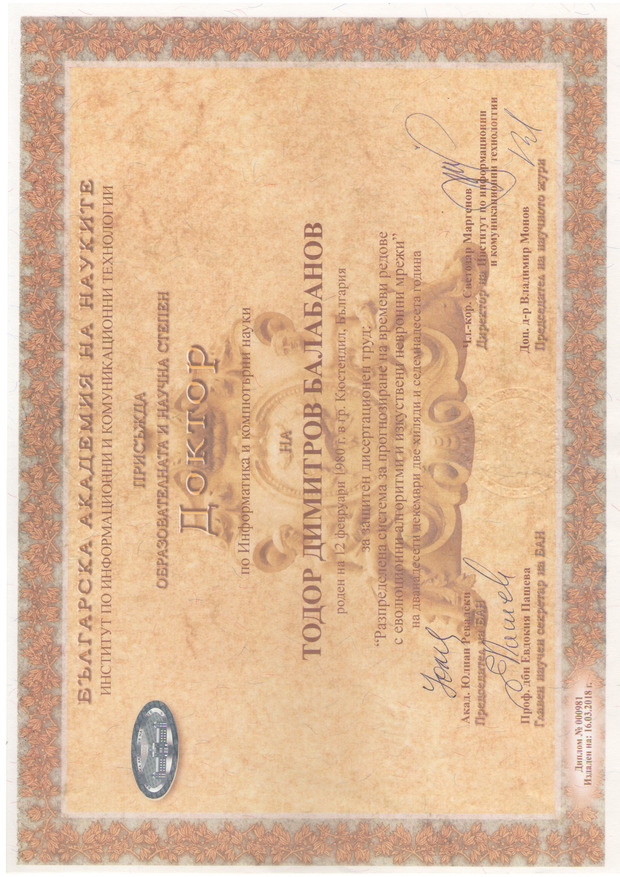
\includegraphics[width=\textwidth,height=\textheight,keepaspectratio]{DiplomaIICT2018}
%
%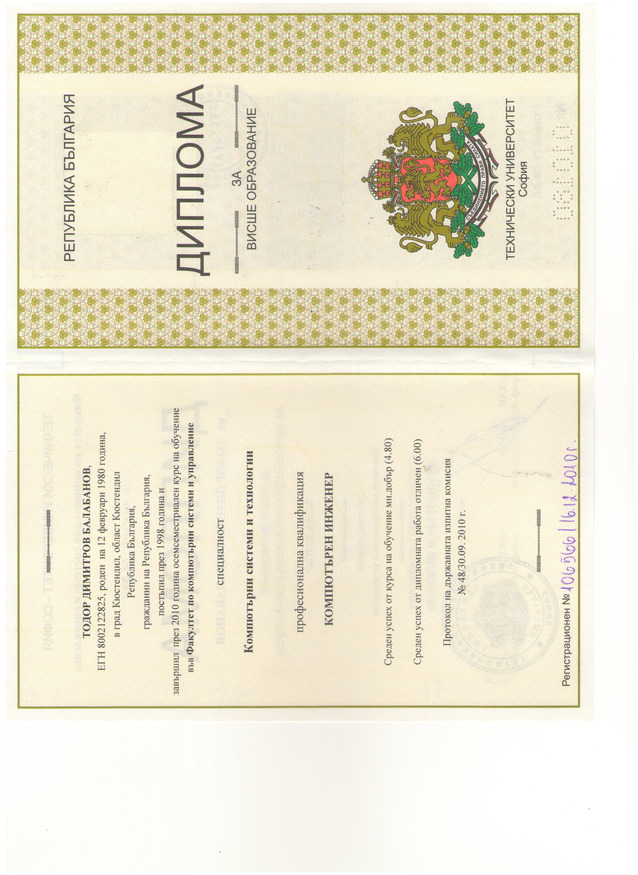
\includegraphics[width=\textwidth,height=\textheight,keepaspectratio]{DiplomaTU2010_1}
%
%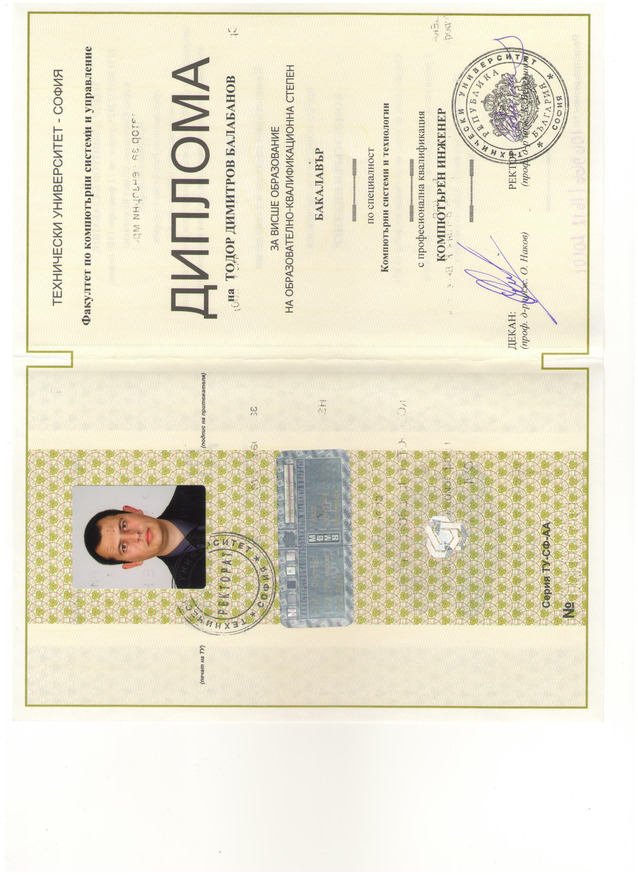
\includegraphics[width=\textwidth,height=\textheight,keepaspectratio]{DiplomaTU2010_2}
%
%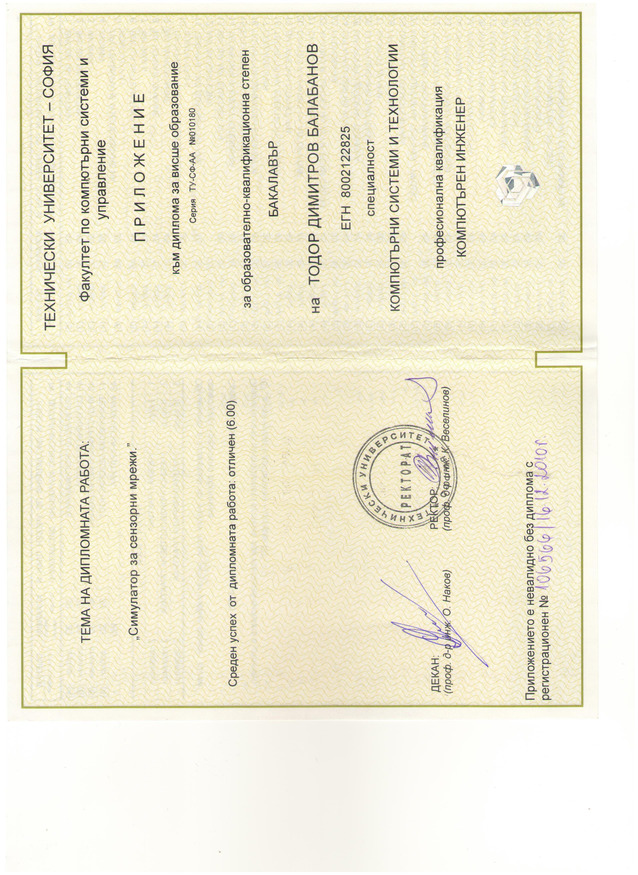
\includegraphics[width=\textwidth,height=\textheight,keepaspectratio]{DiplomaTU2010_3}
%
%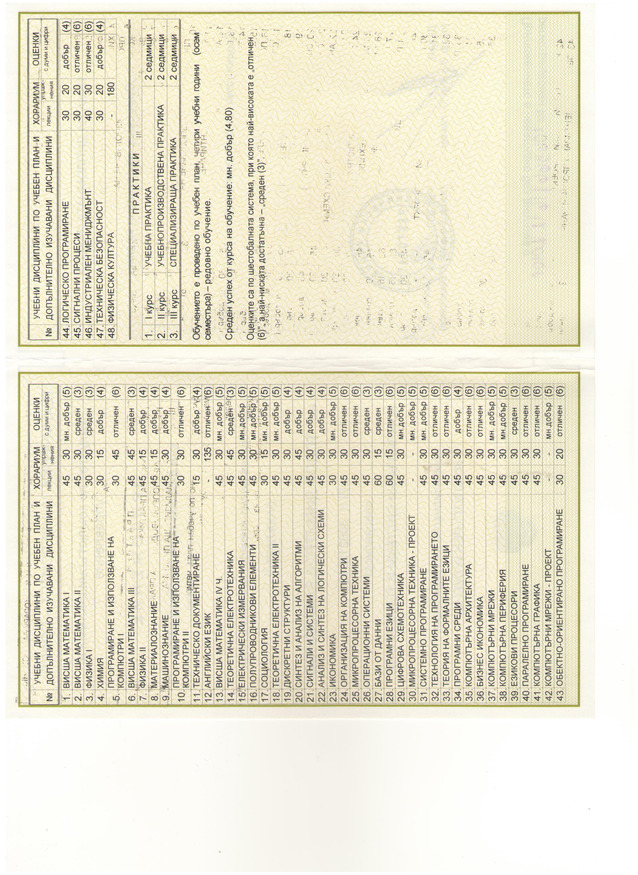
\includegraphics[width=\textwidth,height=\textheight,keepaspectratio]{DiplomaTU2010_4}
%
%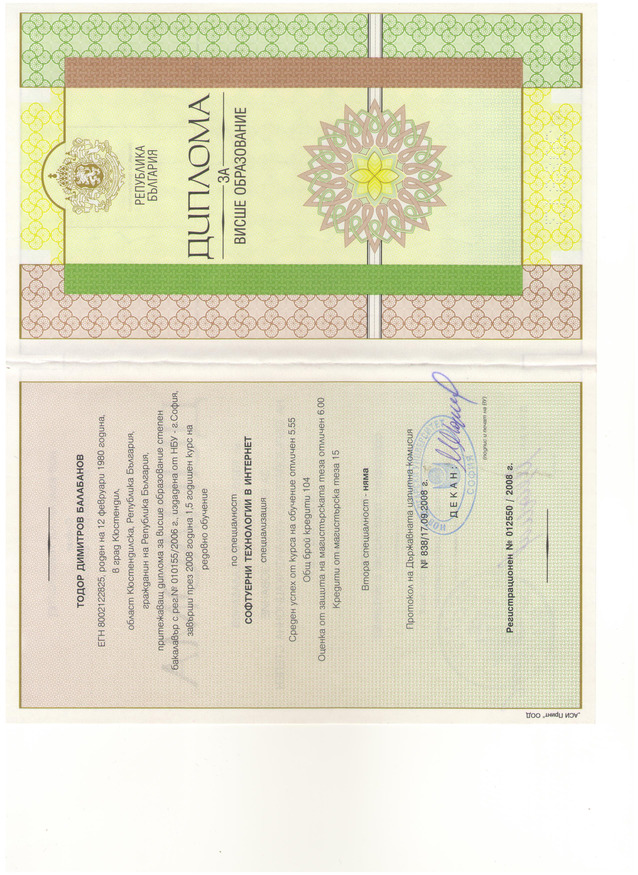
\includegraphics[width=\textwidth,height=\textheight,keepaspectratio]{DiplomaNBU2008_1}
%
%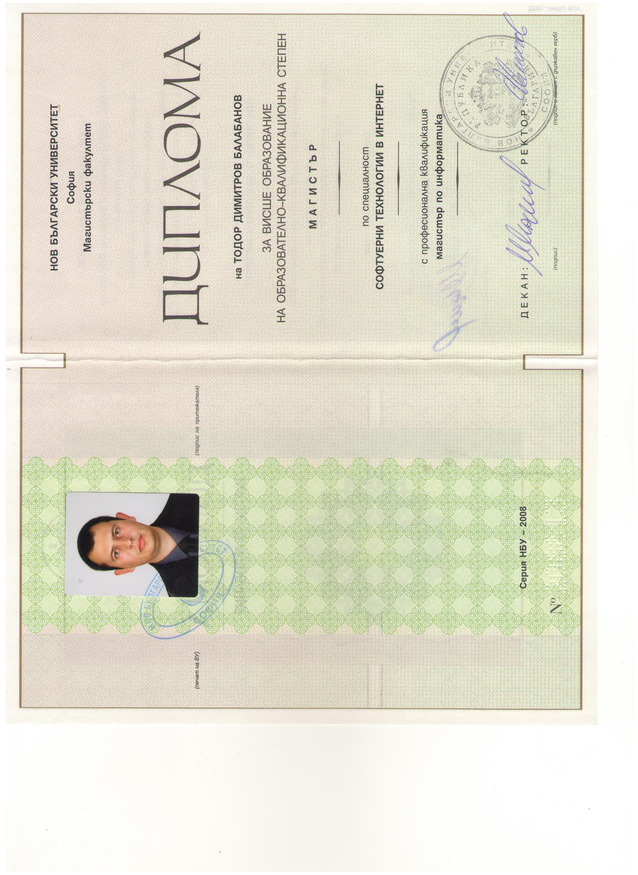
\includegraphics[width=\textwidth,height=\textheight,keepaspectratio]{DiplomaNBU2008_2}
%
%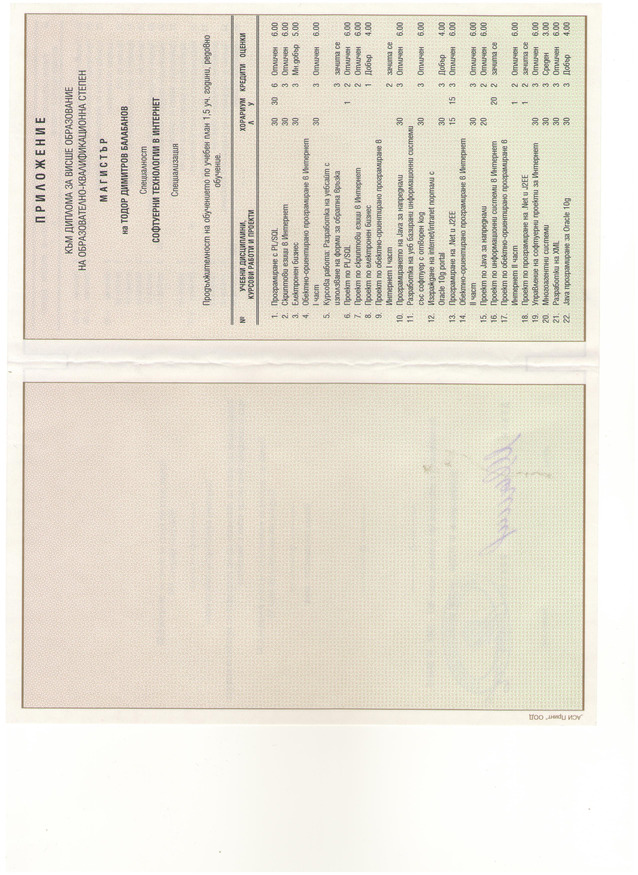
\includegraphics[width=\textwidth,height=\textheight,keepaspectratio]{DiplomaNBU2008_3}
%
%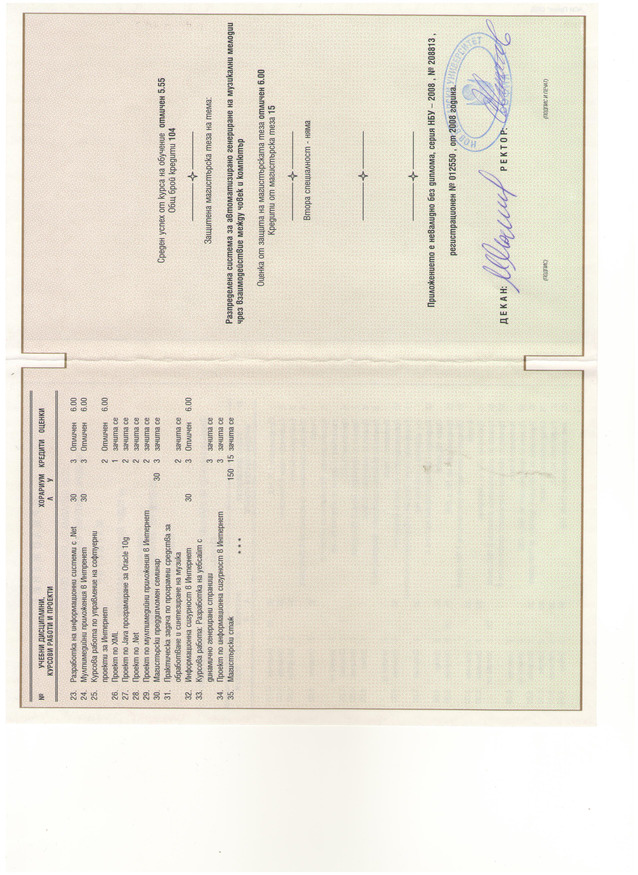
\includegraphics[width=\textwidth,height=\textheight,keepaspectratio]{DiplomaNBU2008_4}
%
%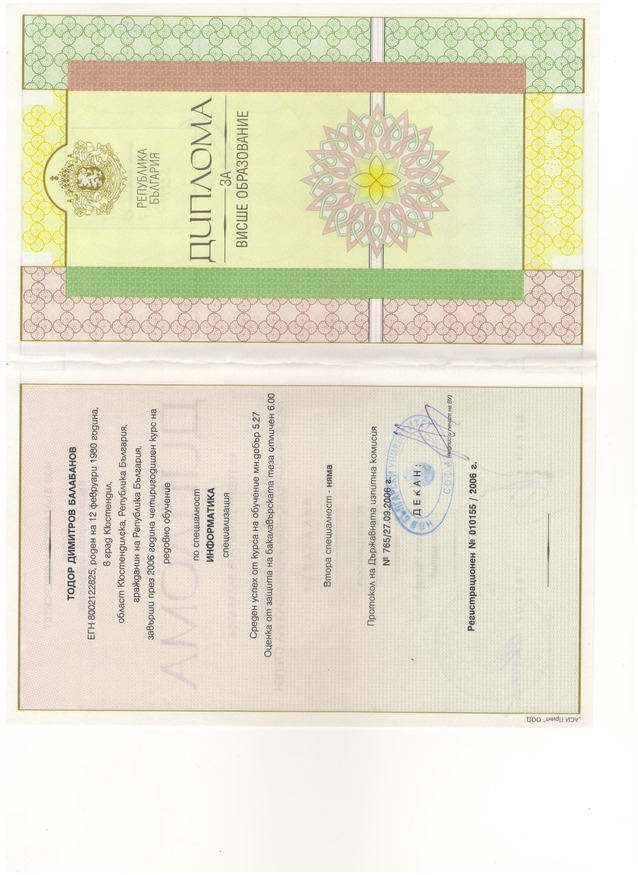
\includegraphics[width=\textwidth,height=\textheight,keepaspectratio]{DiplomaNBU2006_1}
%
%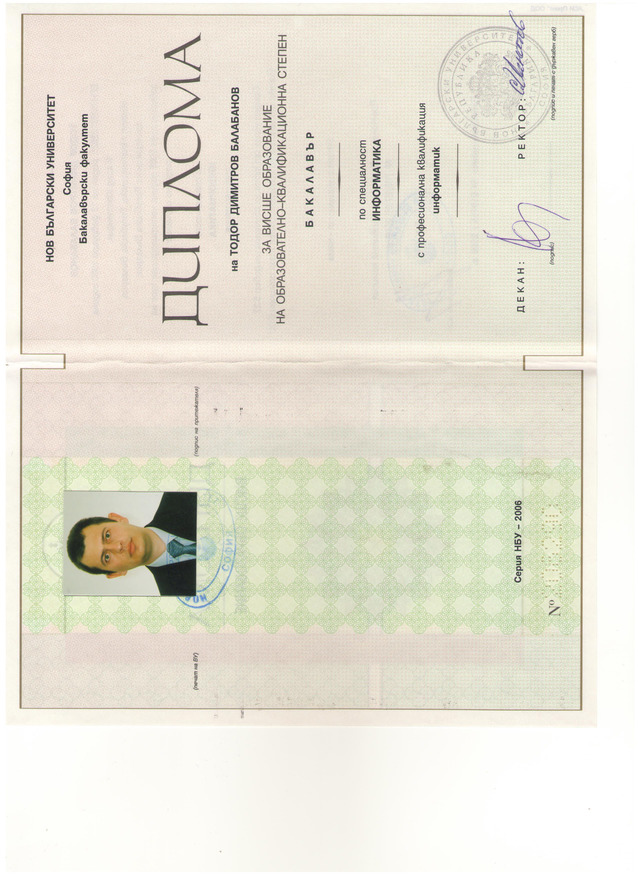
\includegraphics[width=\textwidth,height=\textheight,keepaspectratio]{DiplomaNBU2006_2}
%
%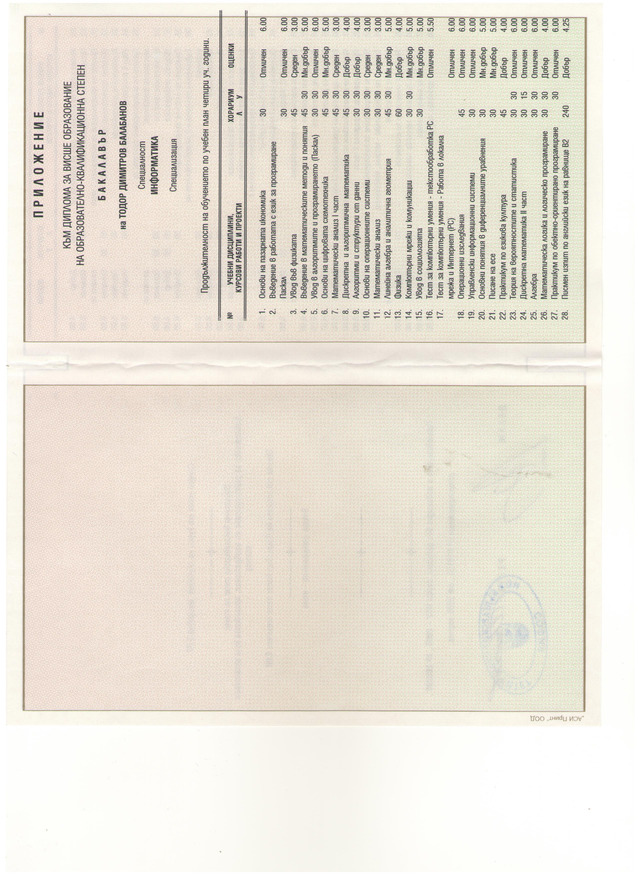
\includegraphics[width=\textwidth,height=\textheight,keepaspectratio]{DiplomaNBU2006_3}
%
%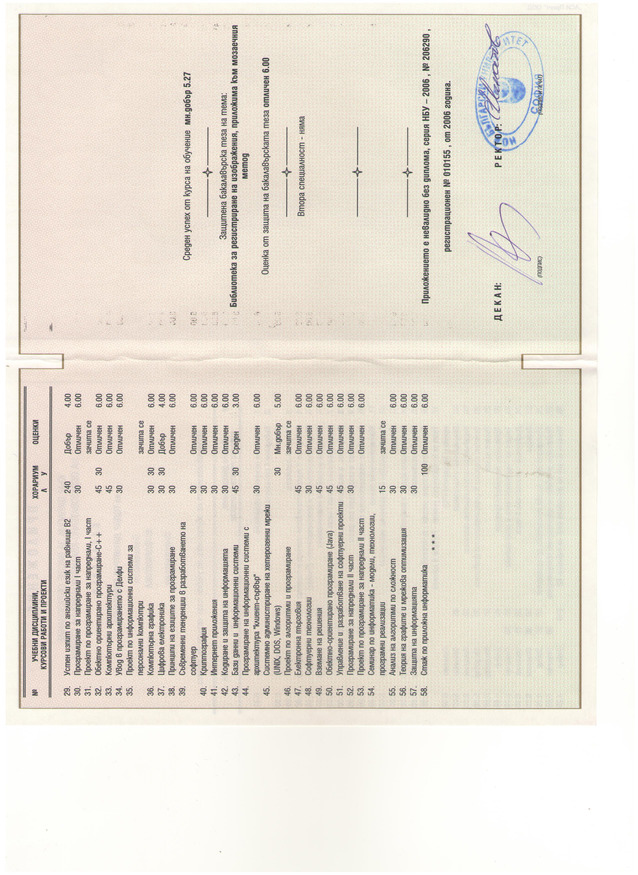
\includegraphics[width=\textwidth,height=\textheight,keepaspectratio]{DiplomaNBU2006_4}
%
%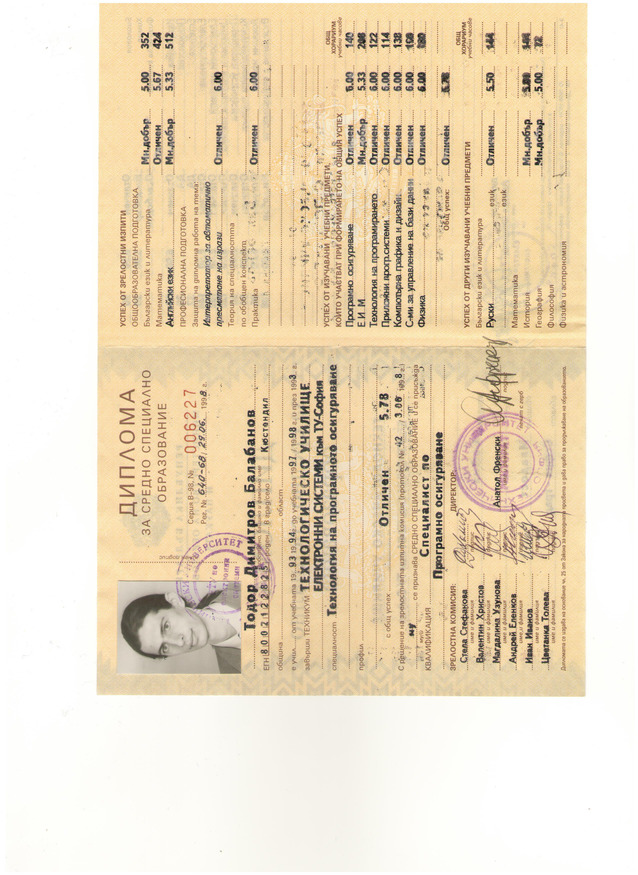
\includegraphics[width=\textwidth,height=\textheight,keepaspectratio]{DiplomaTUES1998_1}
%
%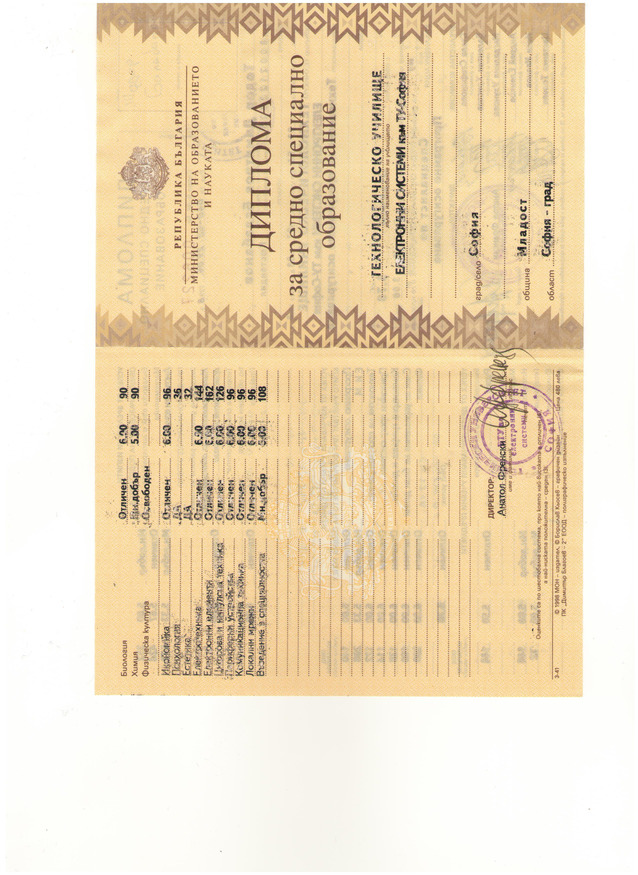
\includegraphics[width=\textwidth,height=\textheight,keepaspectratio]{DiplomaTUES1998_2}
%
%%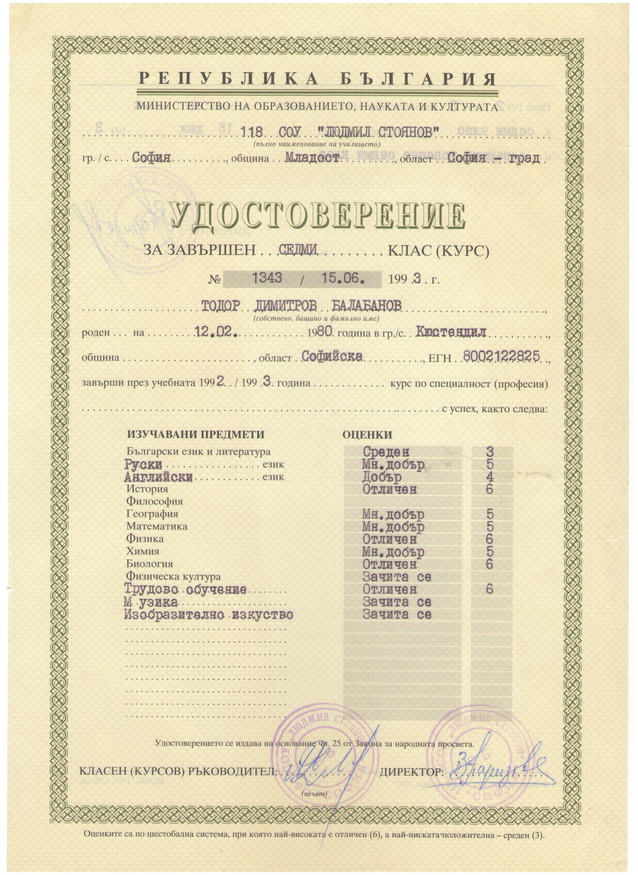
\includegraphics[width=\textwidth,height=\textheight,keepaspectratio]{118SOU1993_1}
%
%%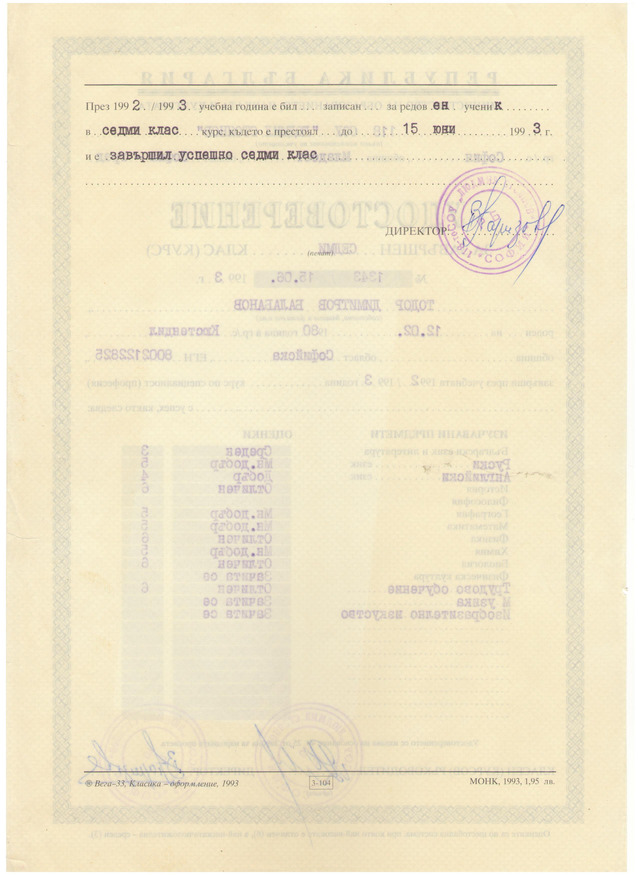
\includegraphics[width=\textwidth,height=\textheight,keepaspectratio]{118SOU1993_2}
%
%%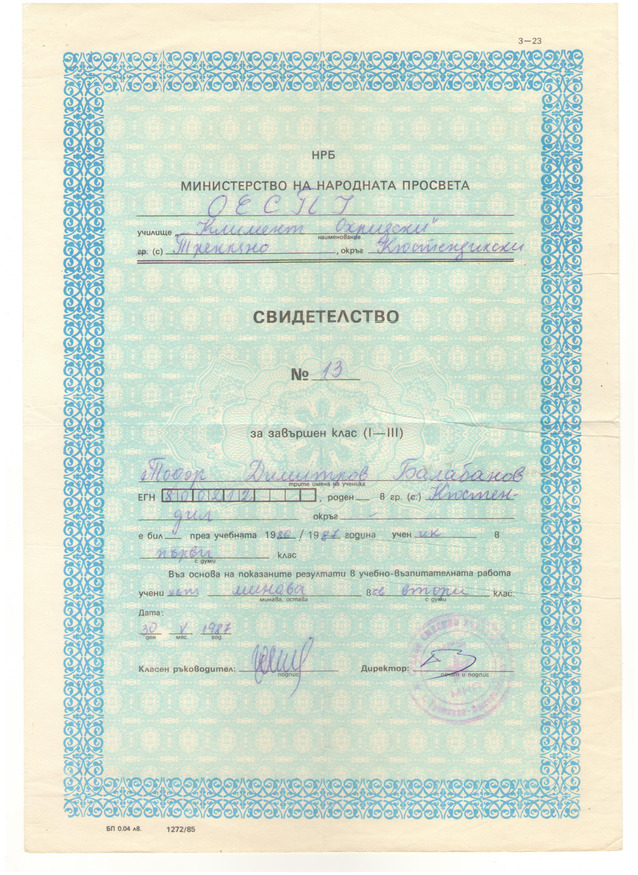
\includegraphics[width=\textwidth,height=\textheight,keepaspectratio]{OESPU1987}
%
%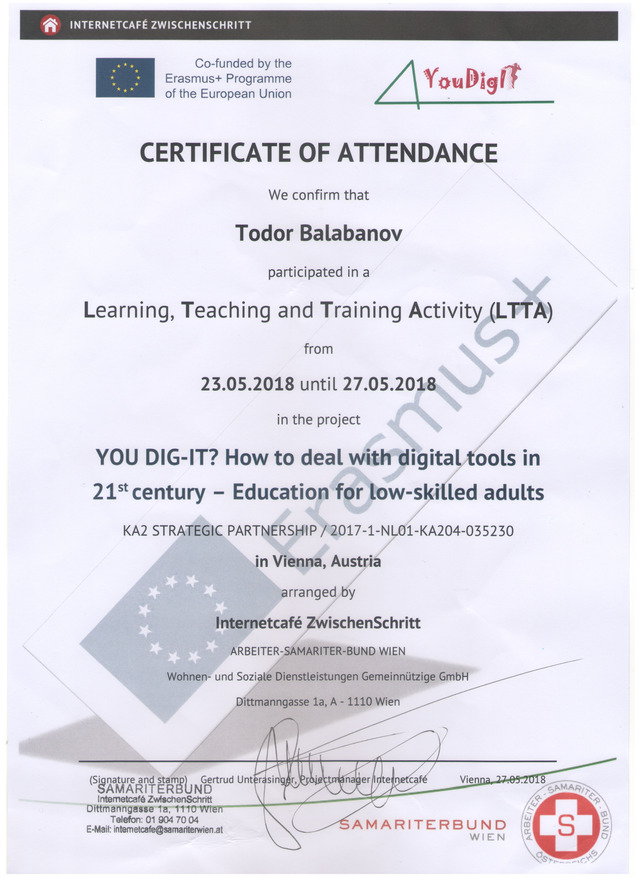
\includegraphics[width=\textwidth,height=\textheight,keepaspectratio]{YouDigIT2018}
%
%
\includegraphics[width=\textwidth,height=\textheight,keepaspectratio]{ESGI1322017}
%
%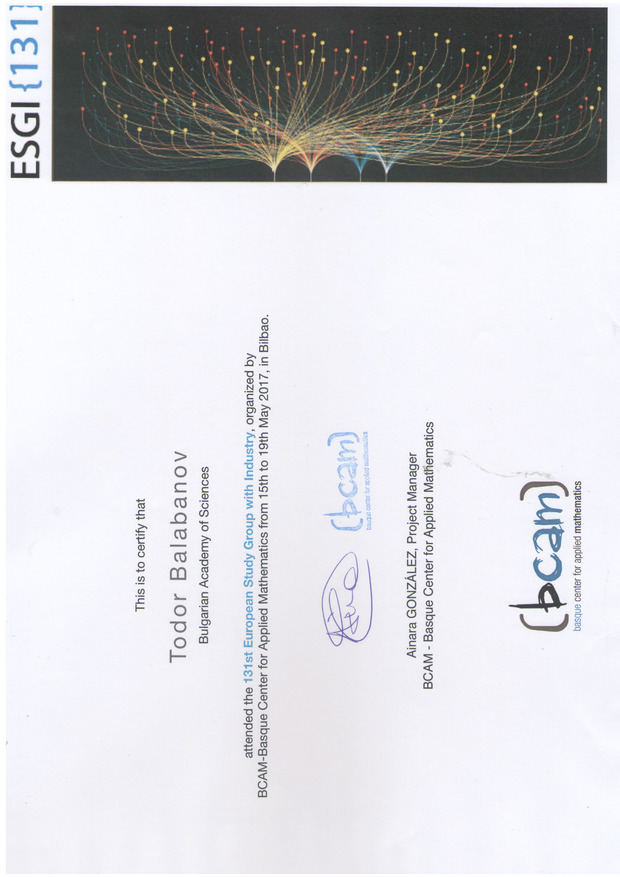
\includegraphics[width=\textwidth,height=\textheight,keepaspectratio]{131ESGI2017}
%
%
\includegraphics[width=\textwidth,height=\textheight,keepaspectratio]{KNSB2017_1}
%
%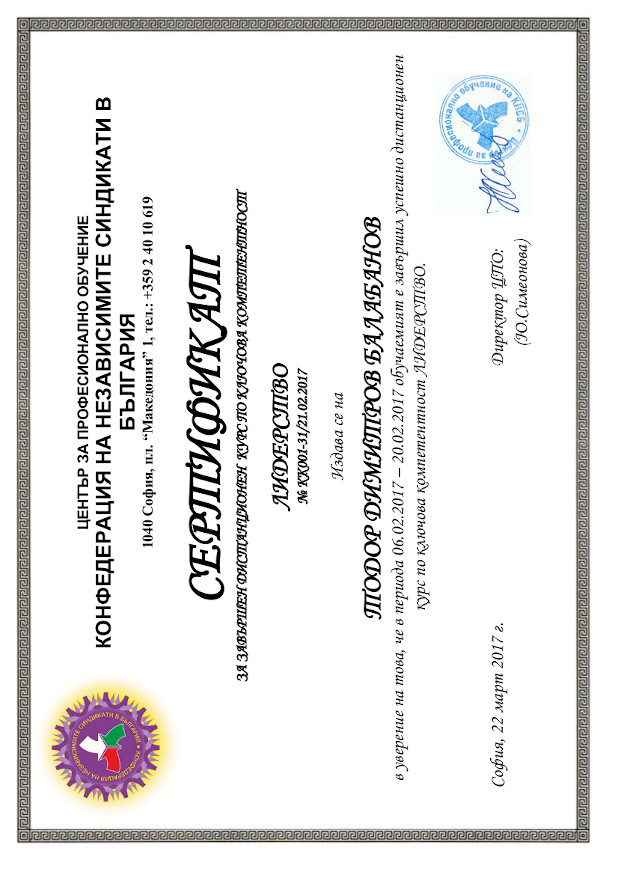
\includegraphics[width=\textwidth,height=\textheight,keepaspectratio]{KNSB2017_2}
%
%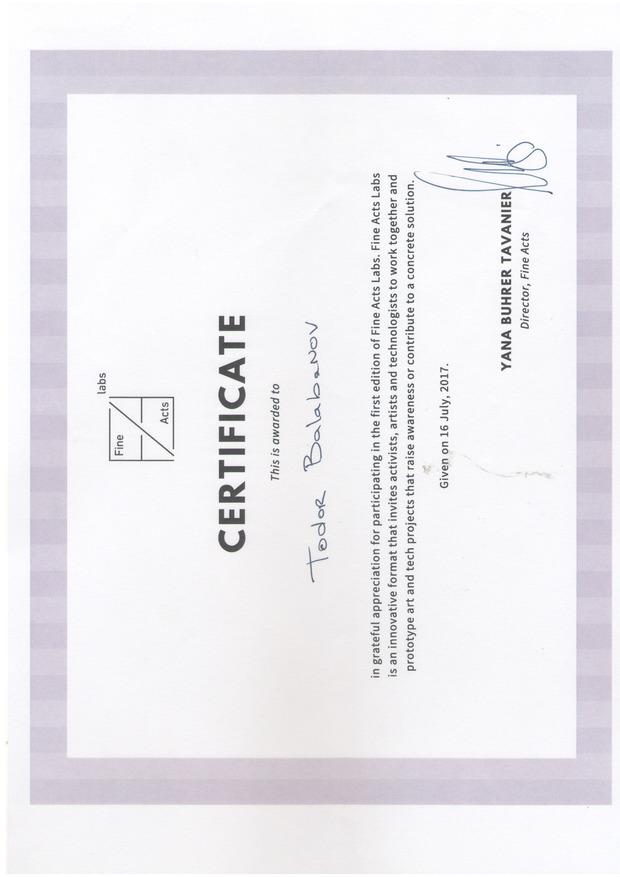
\includegraphics[width=\textwidth,height=\textheight,keepaspectratio]{FineActsLabs2017}
%
%
\includegraphics[width=\textwidth,height=\textheight,keepaspectratio]{InfoTech2016}
%
%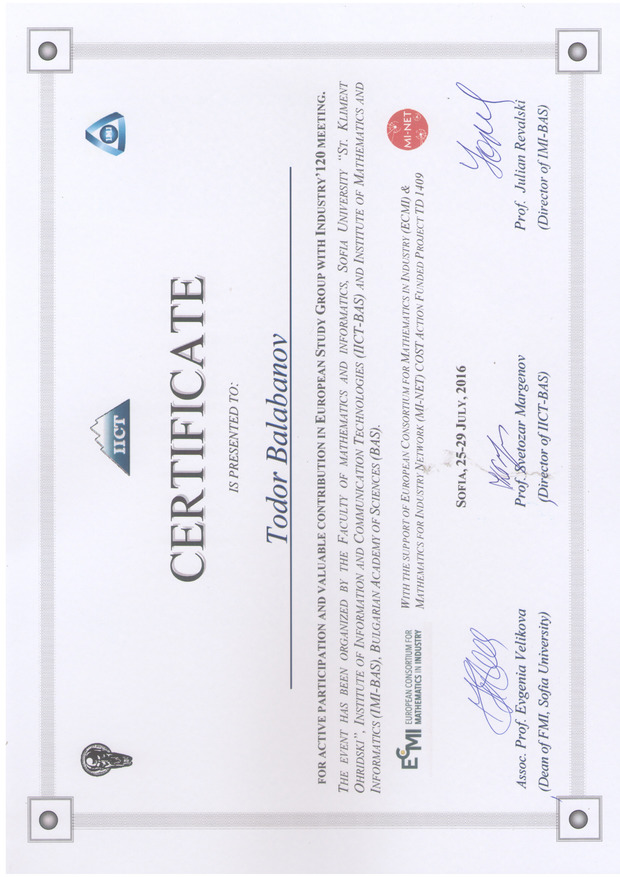
\includegraphics[width=\textwidth,height=\textheight,keepaspectratio]{ESGI1202016}
%
%
\includegraphics[width=\textwidth,height=\textheight,keepaspectratio]{MA2016}
%
%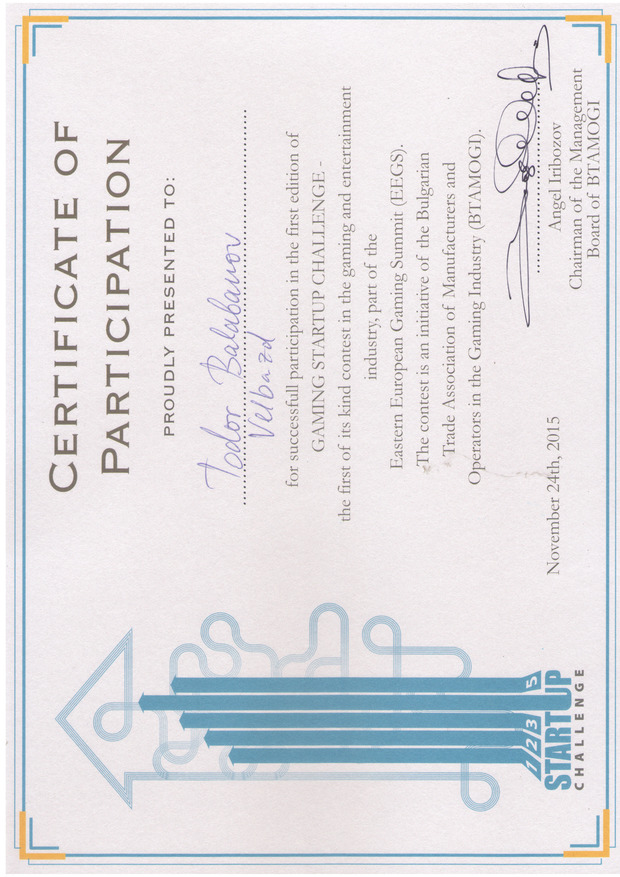
\includegraphics[width=\textwidth,height=\textheight,keepaspectratio]{EEGS2015}
%
%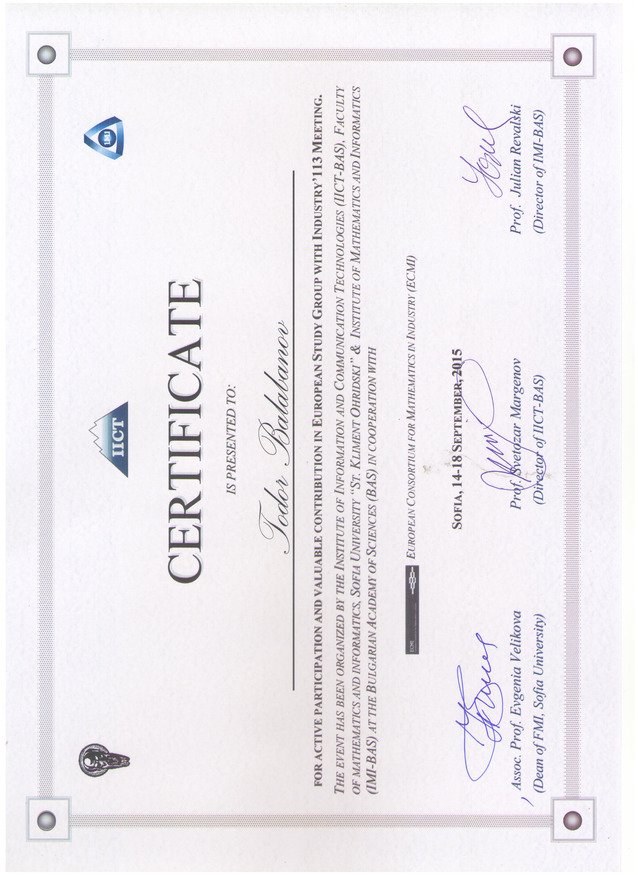
\includegraphics[width=\textwidth,height=\textheight,keepaspectratio]{ESGI1132015}
%
%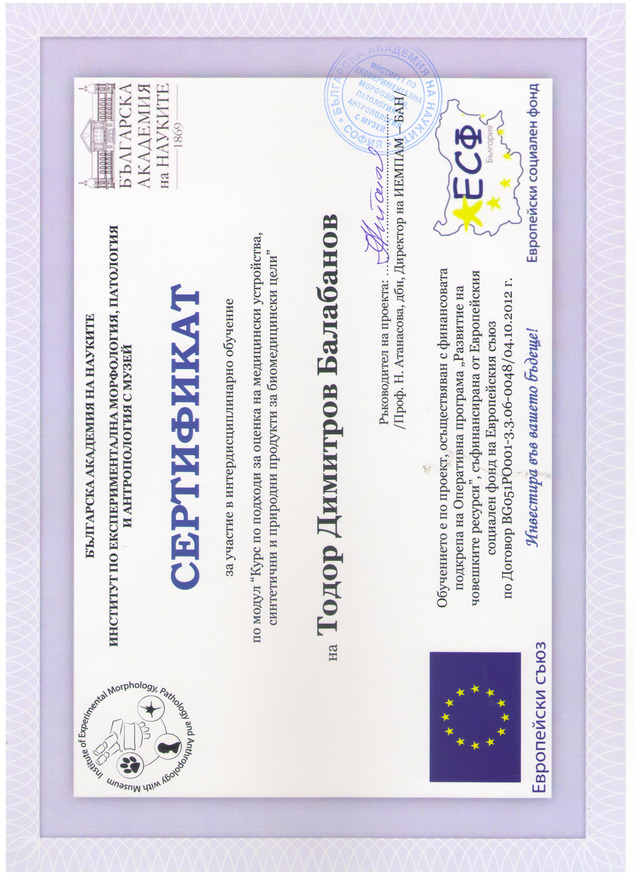
\includegraphics[width=\textwidth,height=\textheight,keepaspectratio]{IEMPAM2014_1}
%
%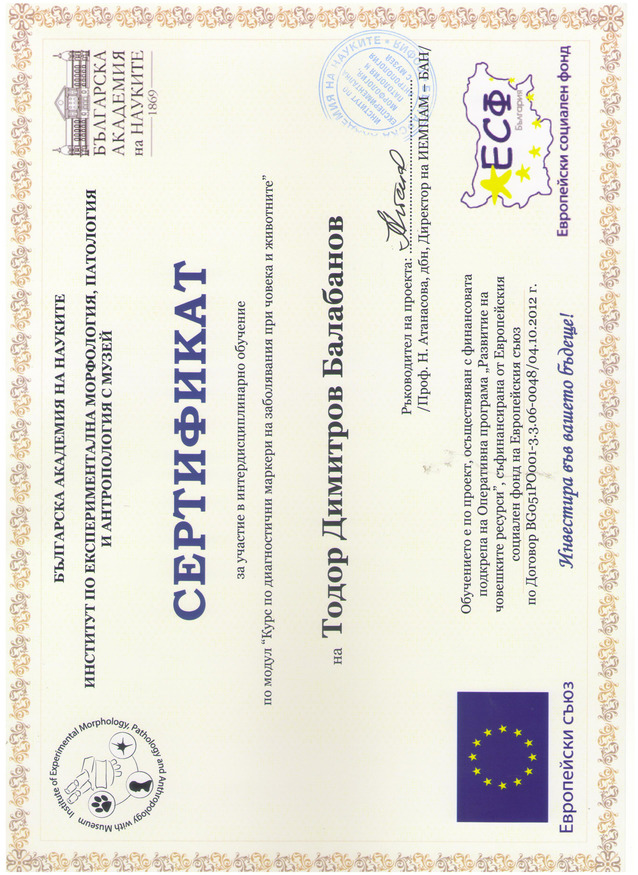
\includegraphics[width=\textwidth,height=\textheight,keepaspectratio]{IEMPAM2014_2}
%
%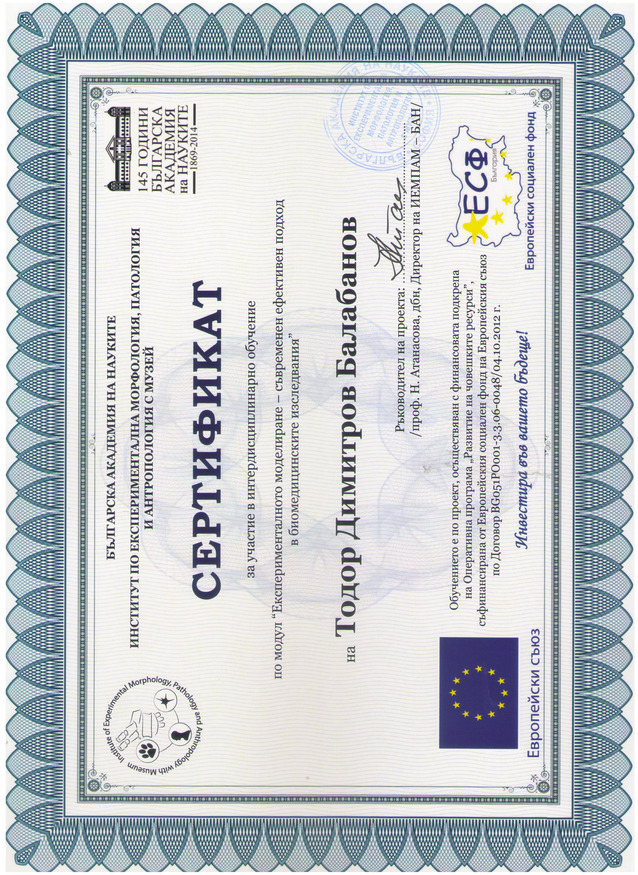
\includegraphics[width=\textwidth,height=\textheight,keepaspectratio]{IEMPAM2014_3}
%
%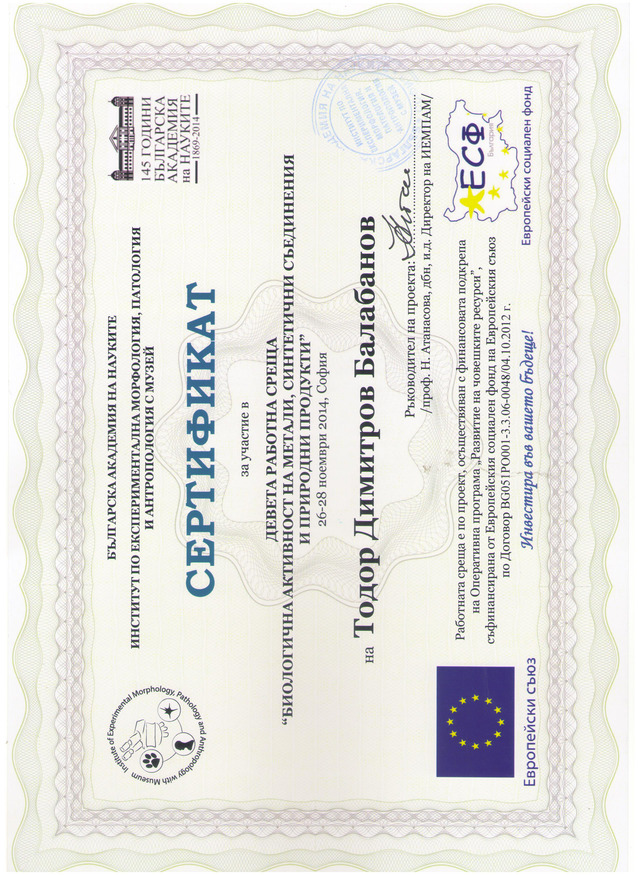
\includegraphics[width=\textwidth,height=\textheight,keepaspectratio]{IEMPAM2014_4}
%
%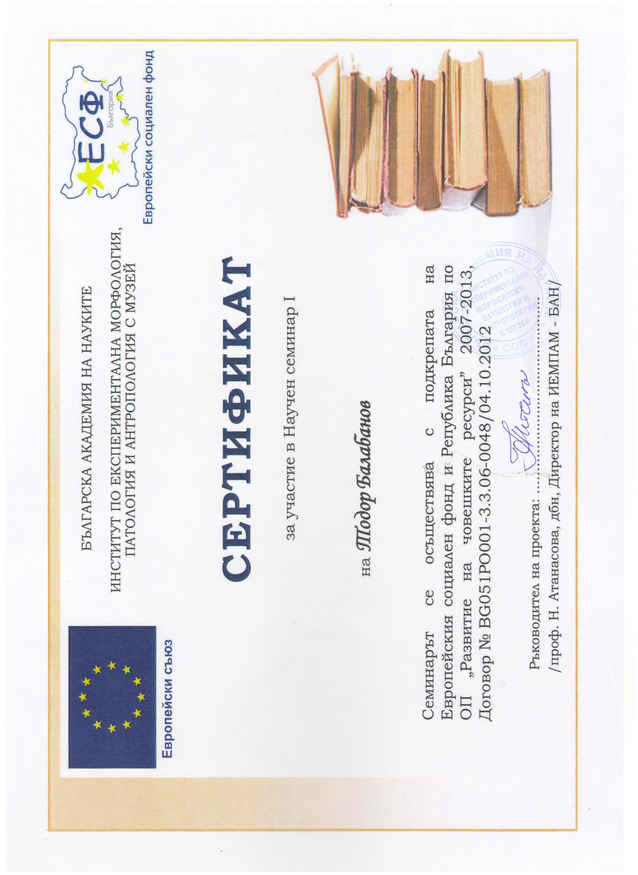
\includegraphics[width=\textwidth,height=\textheight,keepaspectratio]{IEMPAM2013_1}
%
%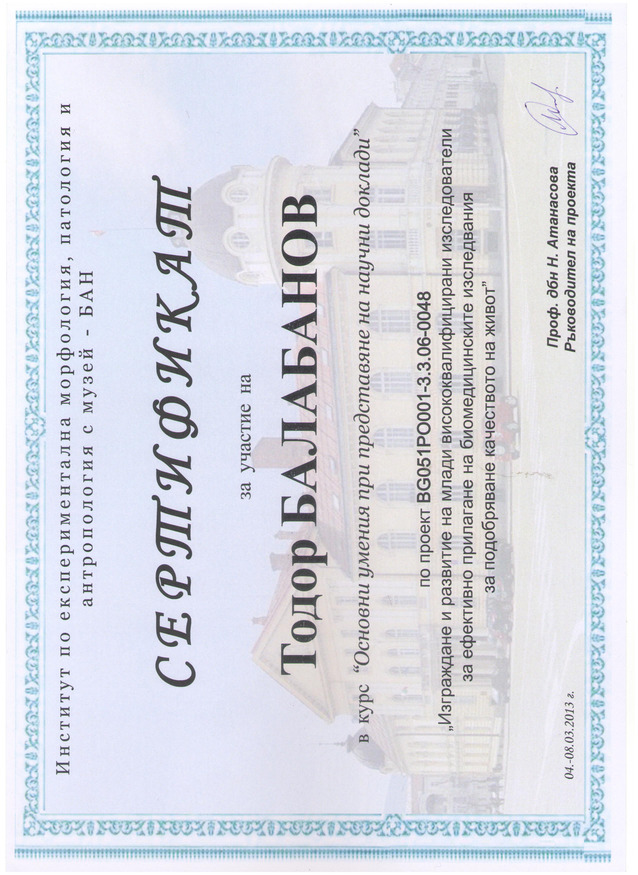
\includegraphics[width=\textwidth,height=\textheight,keepaspectratio]{IEMPAM2013_2}
%
%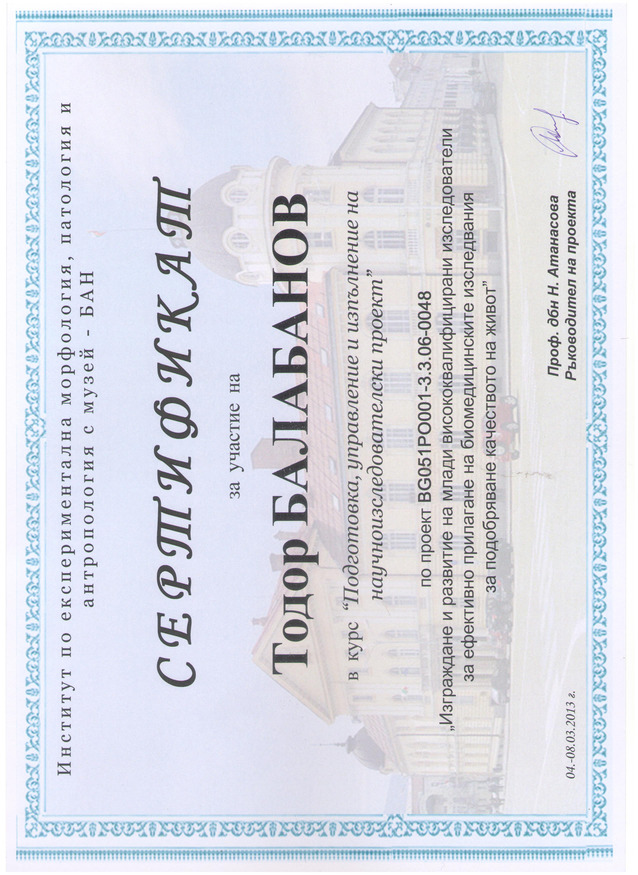
\includegraphics[width=\textwidth,height=\textheight,keepaspectratio]{IEMPAM2013_3}
%
%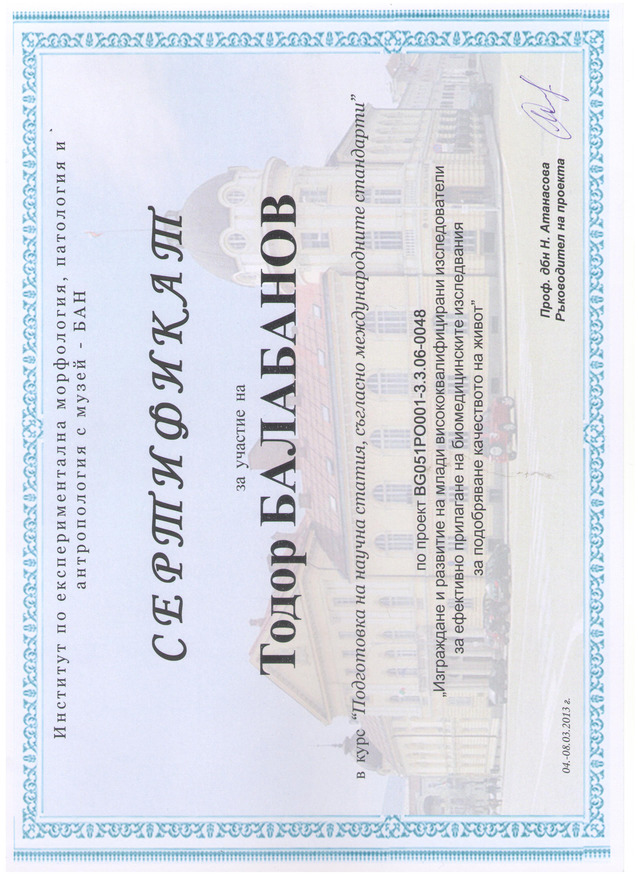
\includegraphics[width=\textwidth,height=\textheight,keepaspectratio]{IEMPAM2013_4}
%
%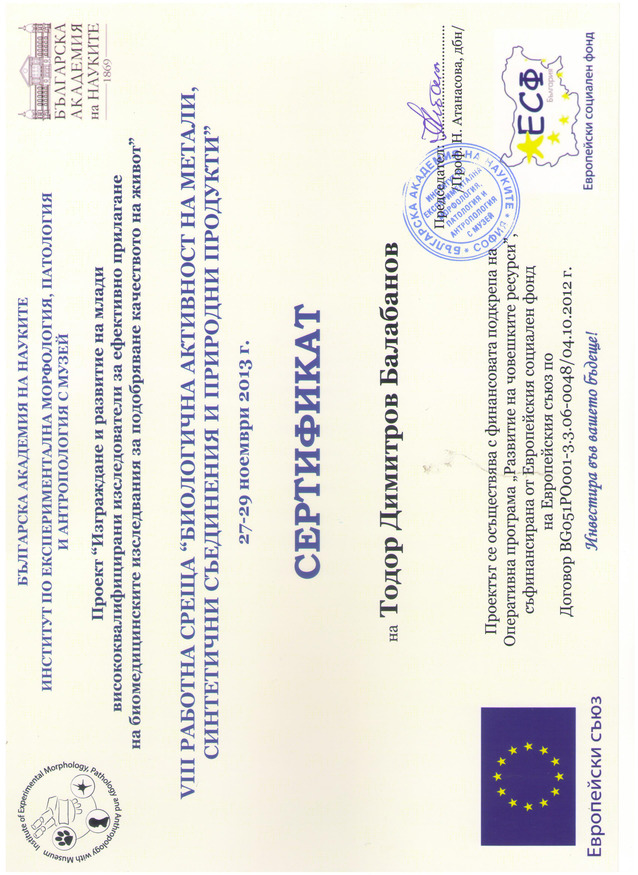
\includegraphics[width=\textwidth,height=\textheight,keepaspectratio]{IEMPAM2013_5}
%
%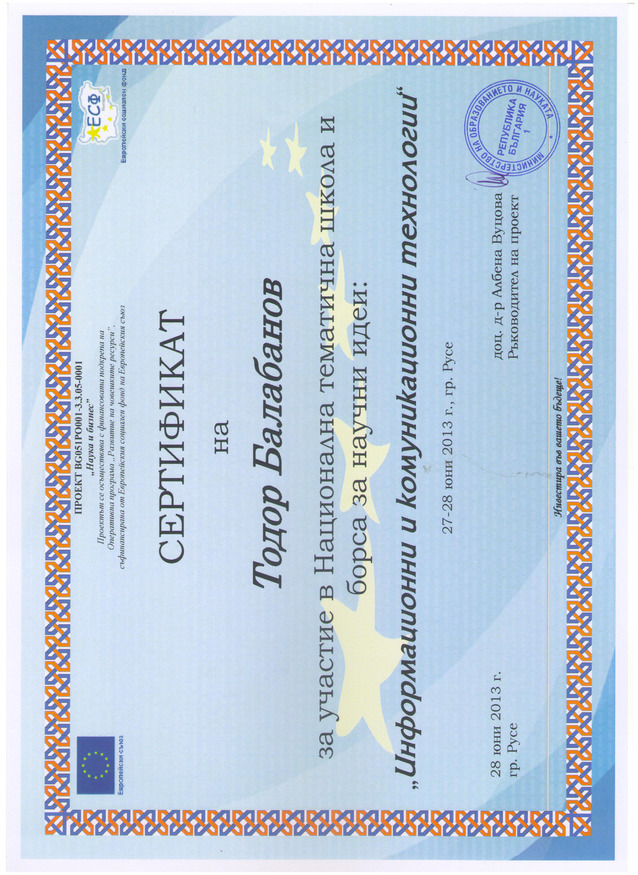
\includegraphics[width=\textwidth,height=\textheight,keepaspectratio]{Rouse2013}
%
%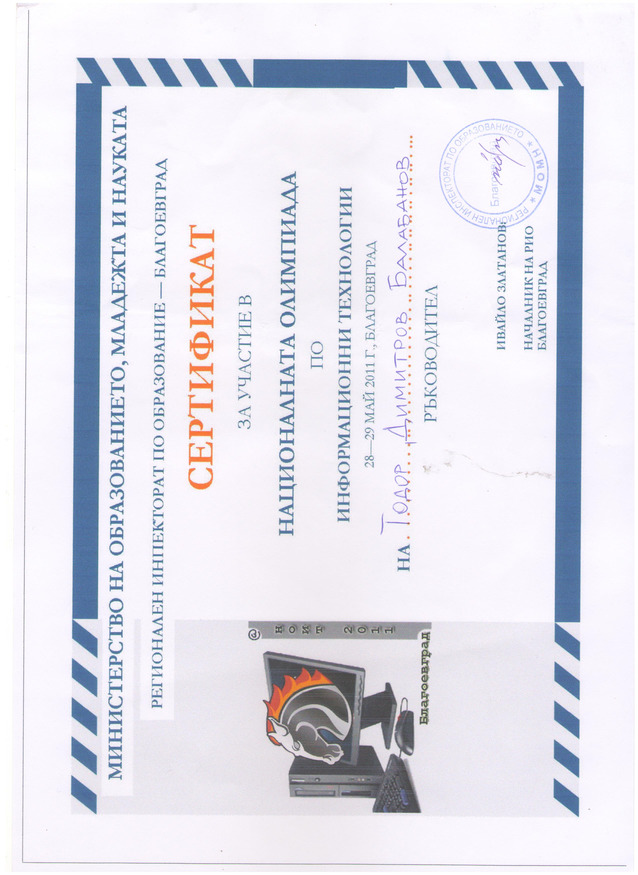
\includegraphics[width=\textwidth,height=\textheight,keepaspectratio]{ElSys2011}
%
%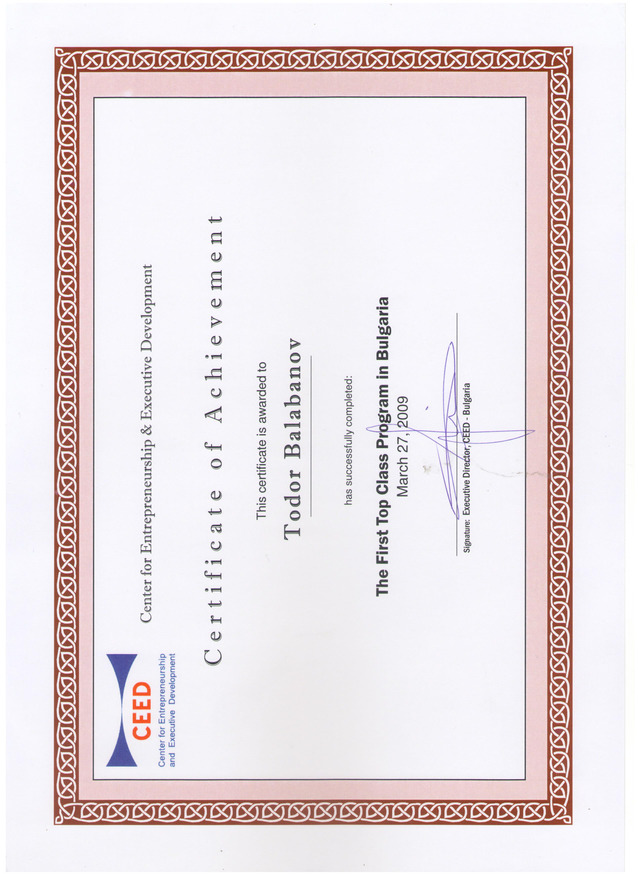
\includegraphics[width=\textwidth,height=\textheight,keepaspectratio]{CEED2009}
%
%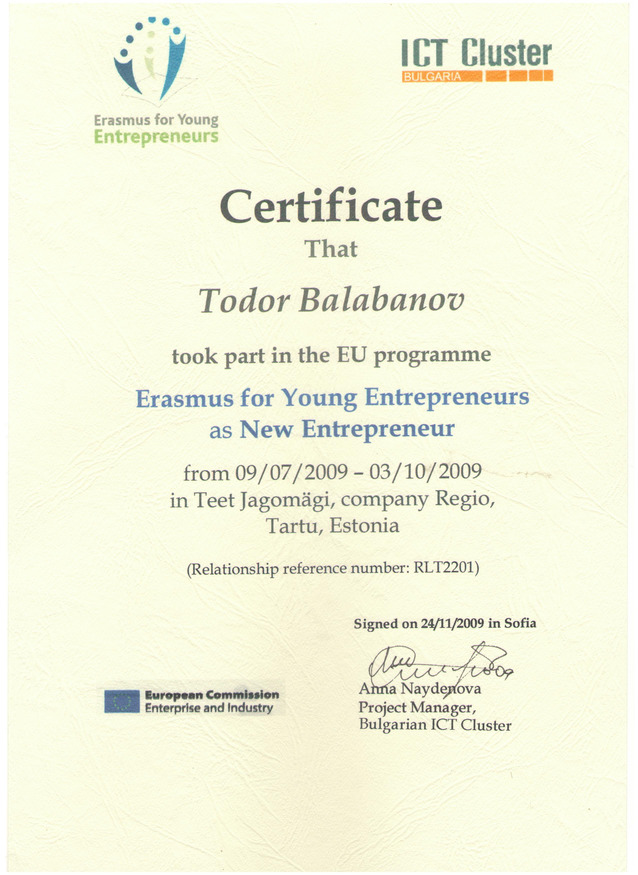
\includegraphics[width=\textwidth,height=\textheight,keepaspectratio]{EYE2009}
%
%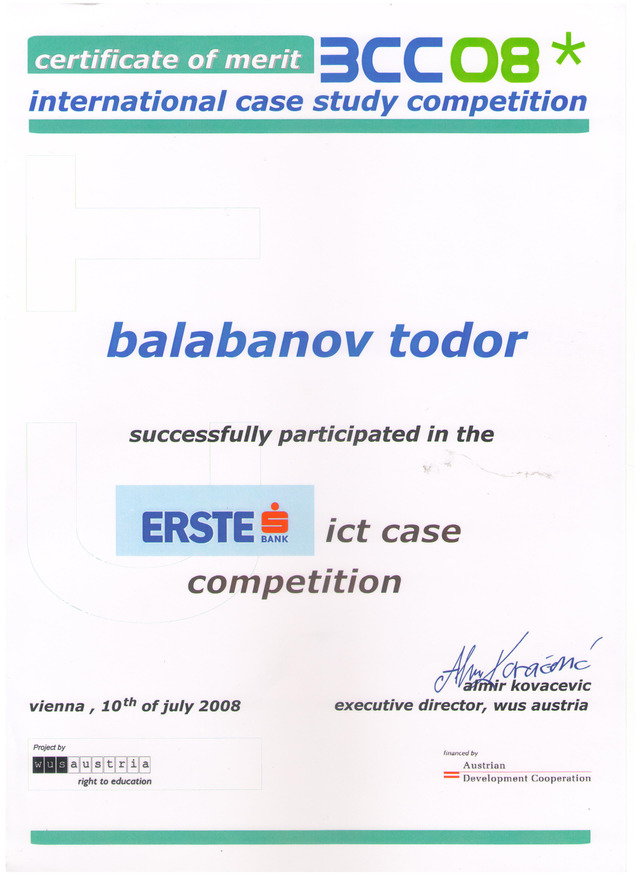
\includegraphics[width=\textwidth,height=\textheight,keepaspectratio]{BCC2008}
%
%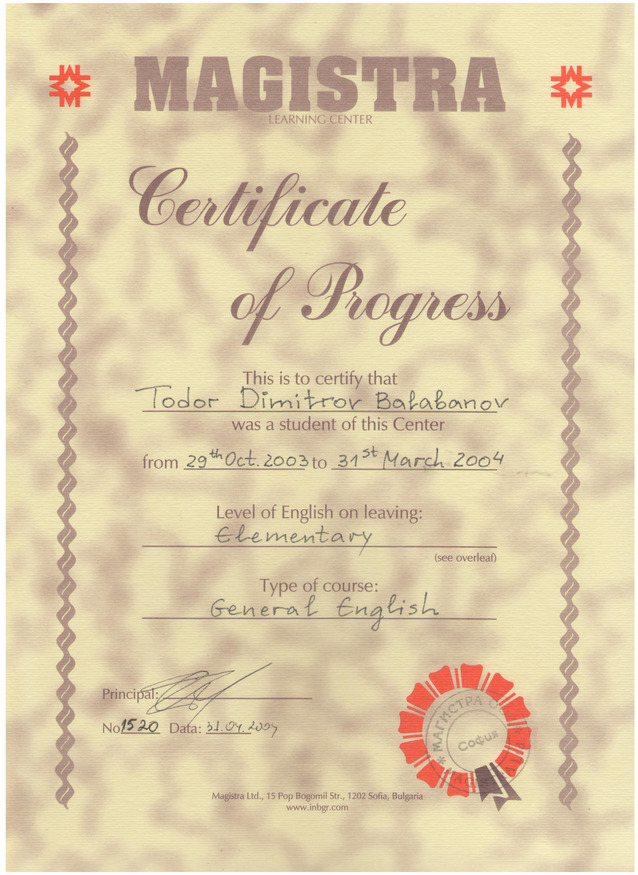
\includegraphics[width=\textwidth,height=\textheight,keepaspectratio]{Magistra2004}
%
%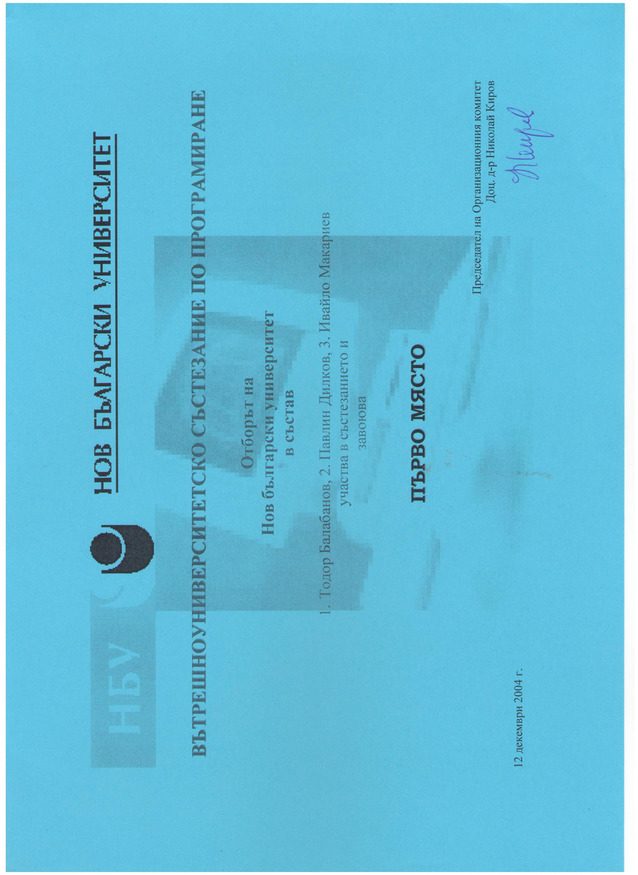
\includegraphics[width=\textwidth,height=\textheight,keepaspectratio]{NBU2004}
%
%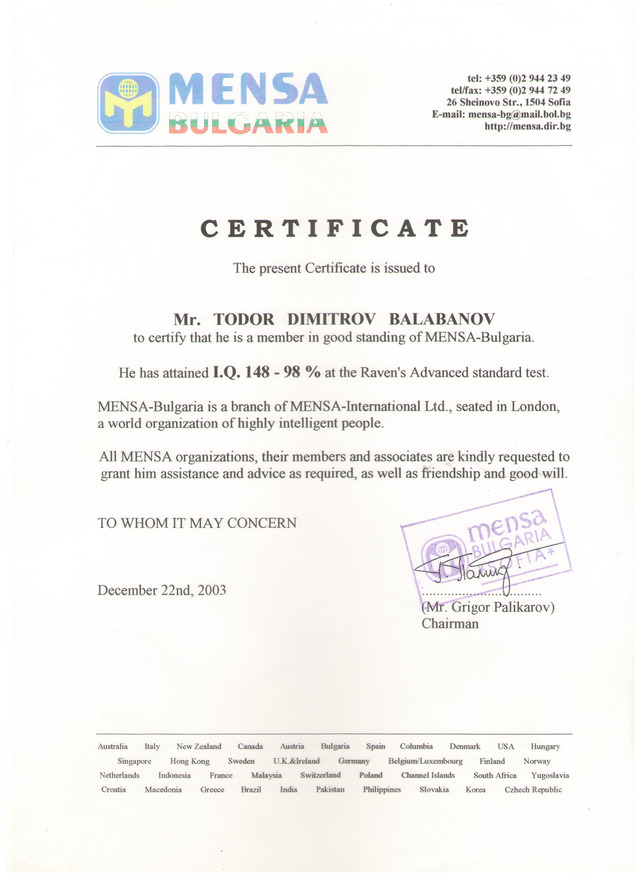
\includegraphics[width=\textwidth,height=\textheight,keepaspectratio]{Mensa2003}
%
%%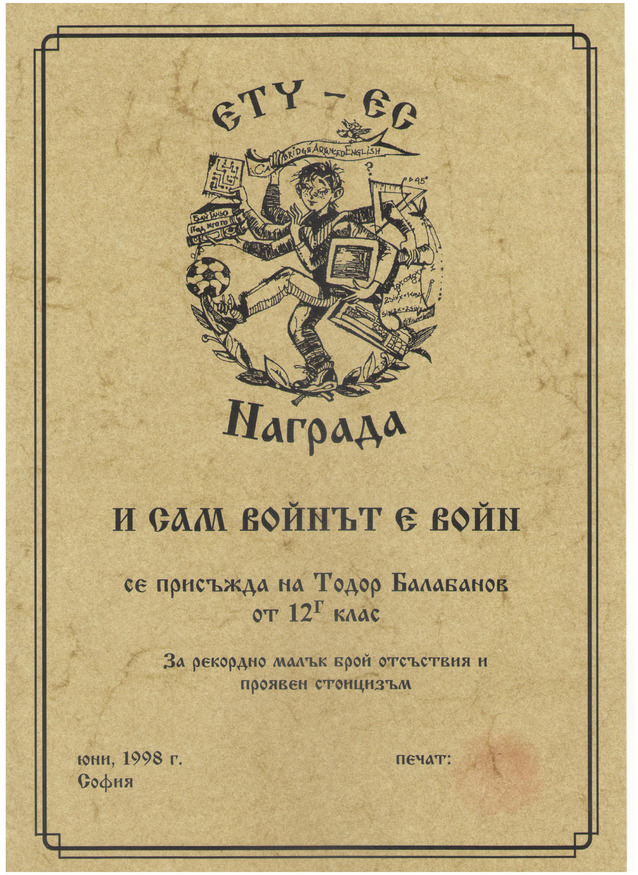
\includegraphics[width=\textwidth,height=\textheight,keepaspectratio]{ElSys1998}
%
%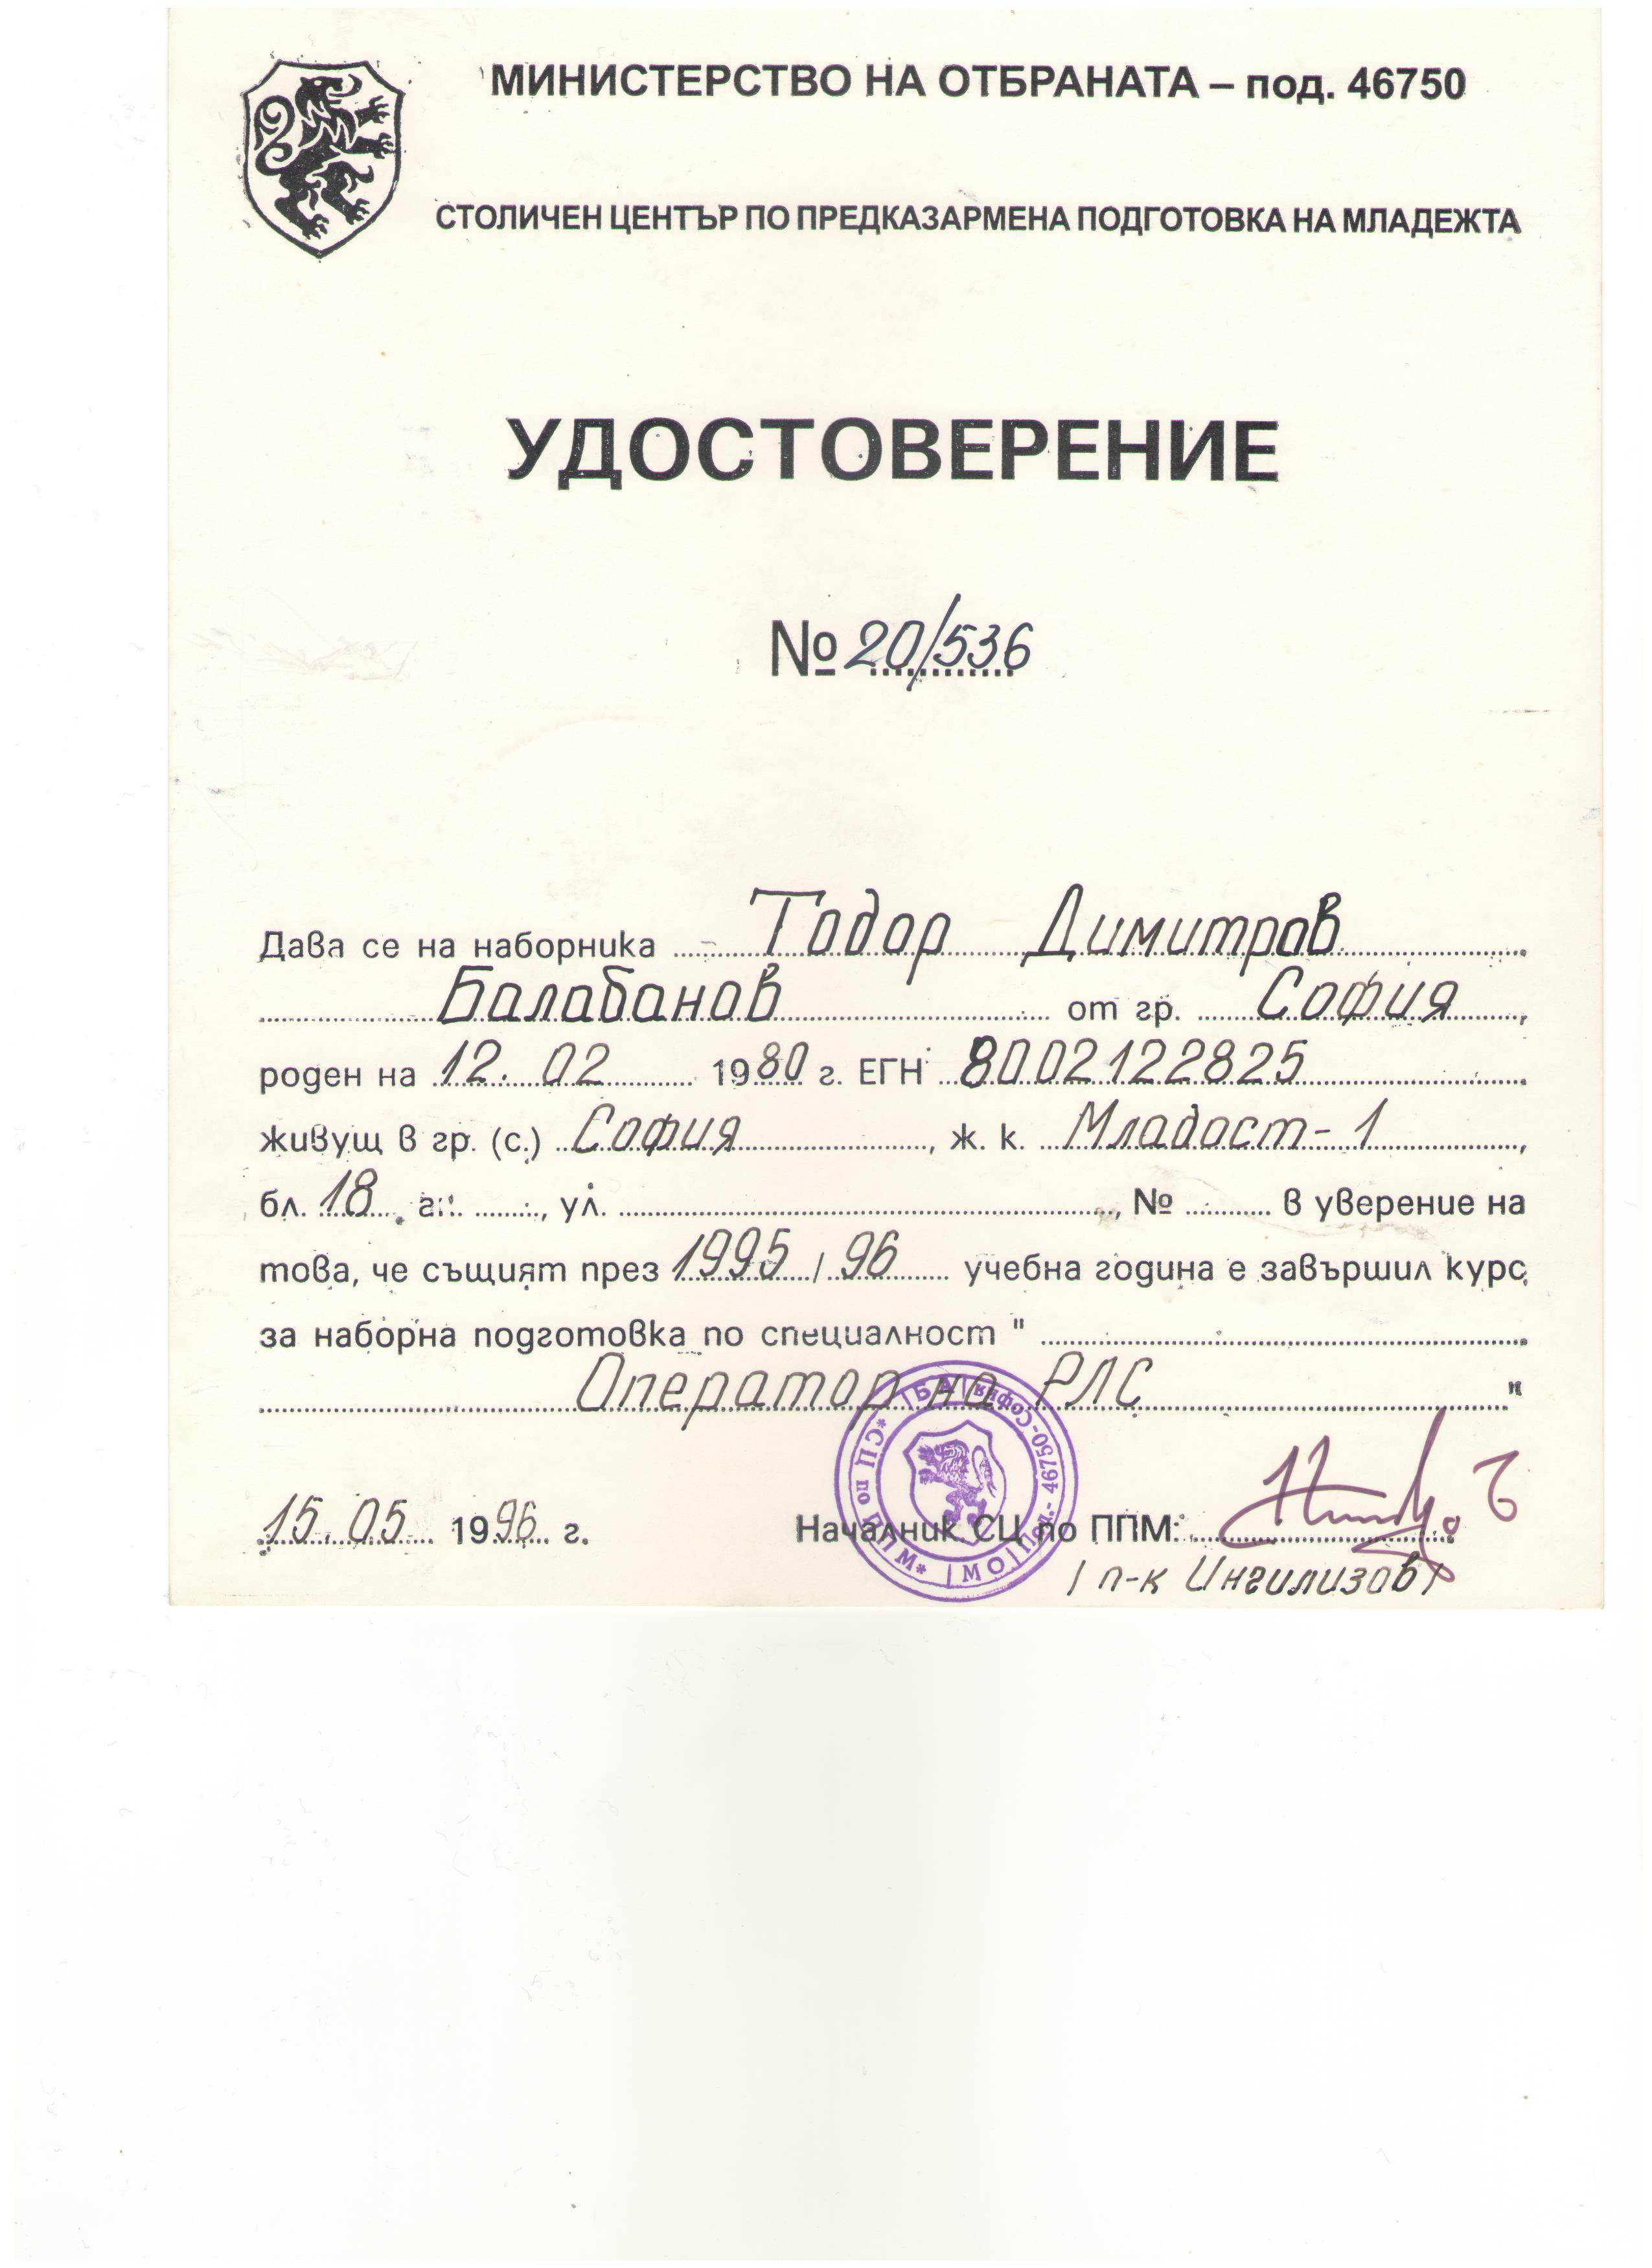
\includegraphics[width=\textwidth,height=\textheight,keepaspectratio]{MO1996}

\end{document}